\begin{center}

\end{center}\section{Power Supply}

\begin{table}[tbh!]
	\caption{Power consumption of KAPTURE-2 components}
	\label{tab:kapturecomp}
	\begin{minipage}{\textwidth}
		\centering
		\begin{tabularx}{\textwidth}{XSSSSS}
			\toprule
			\textbf{Component} & \textbf{$V_{cc}$ (\SI{}{\volt})} & \textbf{$I_{max}$ (\SI{}{\ampere})} & \textbf{$P_{max}$ (\SI{}{\watt})} & $\#_{parts}$ & \textbf{$I_{tot}$}\footnote{for 16 ADCs} (\SI{}{\ampere})\\
				\midrule
			HMC5649 (T/H-Amplifier) 	& 2	  	& 0.221 	 & 0.442 & 16 & 3.536\\
									& -5  	& -0.242 & 1.21 &  & 3.872\\
			HMC856 (Delay) 			& -3.3	& 0.185 & -0.611 & 16 & 2.96\\
			HMC987LP5E (Fan-Out) 	& 3.3 	& 0.234\footnote{All Outputs and RF-Buffer} & 0.772 & 2 & 0.468\\
			LMC0480 (PLL) 			& 3.3 	& 0.590\footnote{All CLKs} & 1.947 & ? & ???\\
			VCXO 					& 3.3 	& 0.03 & 0.198 & ? & ???\\
			\bottomrule
		\end{tabularx}
	\end{minipage}
\end{table}

\paragraph{PLL LMK0480}
The LMK0480 is used for jitter cleaning of the clock signal coming from KARA. It feeds to the FanOut, FPGA and -- in KAPTURE-2 -- to the ADCs.
\begin{itemize}
	\item Number of CLKOuts: 11
	\item CLKOuts are grouped together as follows
	\begin{table}[tbh!]
	\caption{CLKOut Groups of PLL LMK0480}
	\label{tab:pll}
	\begin{minipage}{\textwidth}
		\centering
		\begin{tabularx}{0.5\textwidth}{cc}
			\toprule
			\textbf{Clock Group} & \textbf{Clock Outputs} \\
				\midrule
			0	& CLKout0, CLKout1\\
			1	& CLKout2, CLKout3\\
			2	& CLKout4, CLKout5\\
			3	& CLKout6, CLKout7\\
			4	& CLKout8, CLKout9\\
			5	& CLKout10, CLKout11\\
			\bottomrule
		\end{tabularx}
	\end{minipage}
\end{table}
	\item Adjustable delay at CLKouts: 
	\begin{itemize}
		\item \textbf{Fine, analog delay}: Step size \SI{25}{\pico\second}, range from 0 to \SI{475}{\pico \second} \newline 
		$\rightarrow$ Enabling adds a nominal \SI{500}{\pico\second} of delay in addition to the programmed value.
		\item \textbf{Coarse, digital delay}: Delay of 4.5 to 12 clock distribution path cycles (normal mode) or 12.5 to 522 VCO cycles (extended mode) $\rightarrow$ step as small as half of period of clock distribution path cycle (using \texttt{CLKoutX\_Y\_HS} bit, when output divide value > 1)
	\end{itemize}

\item Fixed digital delay is determined by the frequency of distribution path. With an external VCO the resolution (one delay step) is determined by: 
	\begin{equation}
		DD_{Res}=\frac{1}{2\times VCO\_Frequency}
	\end{equation}
	For a desired delay \texttt{CLKX\_Y\_DDLY} and \texttt{CLKX\_Y\_HS} have to be set accordingly, with \texttt{X} being the even and \texttt{Y} being the odd number of the \texttt{CLKout} in the group.
\end{itemize}


\begin{figure}[H]
	\centering
	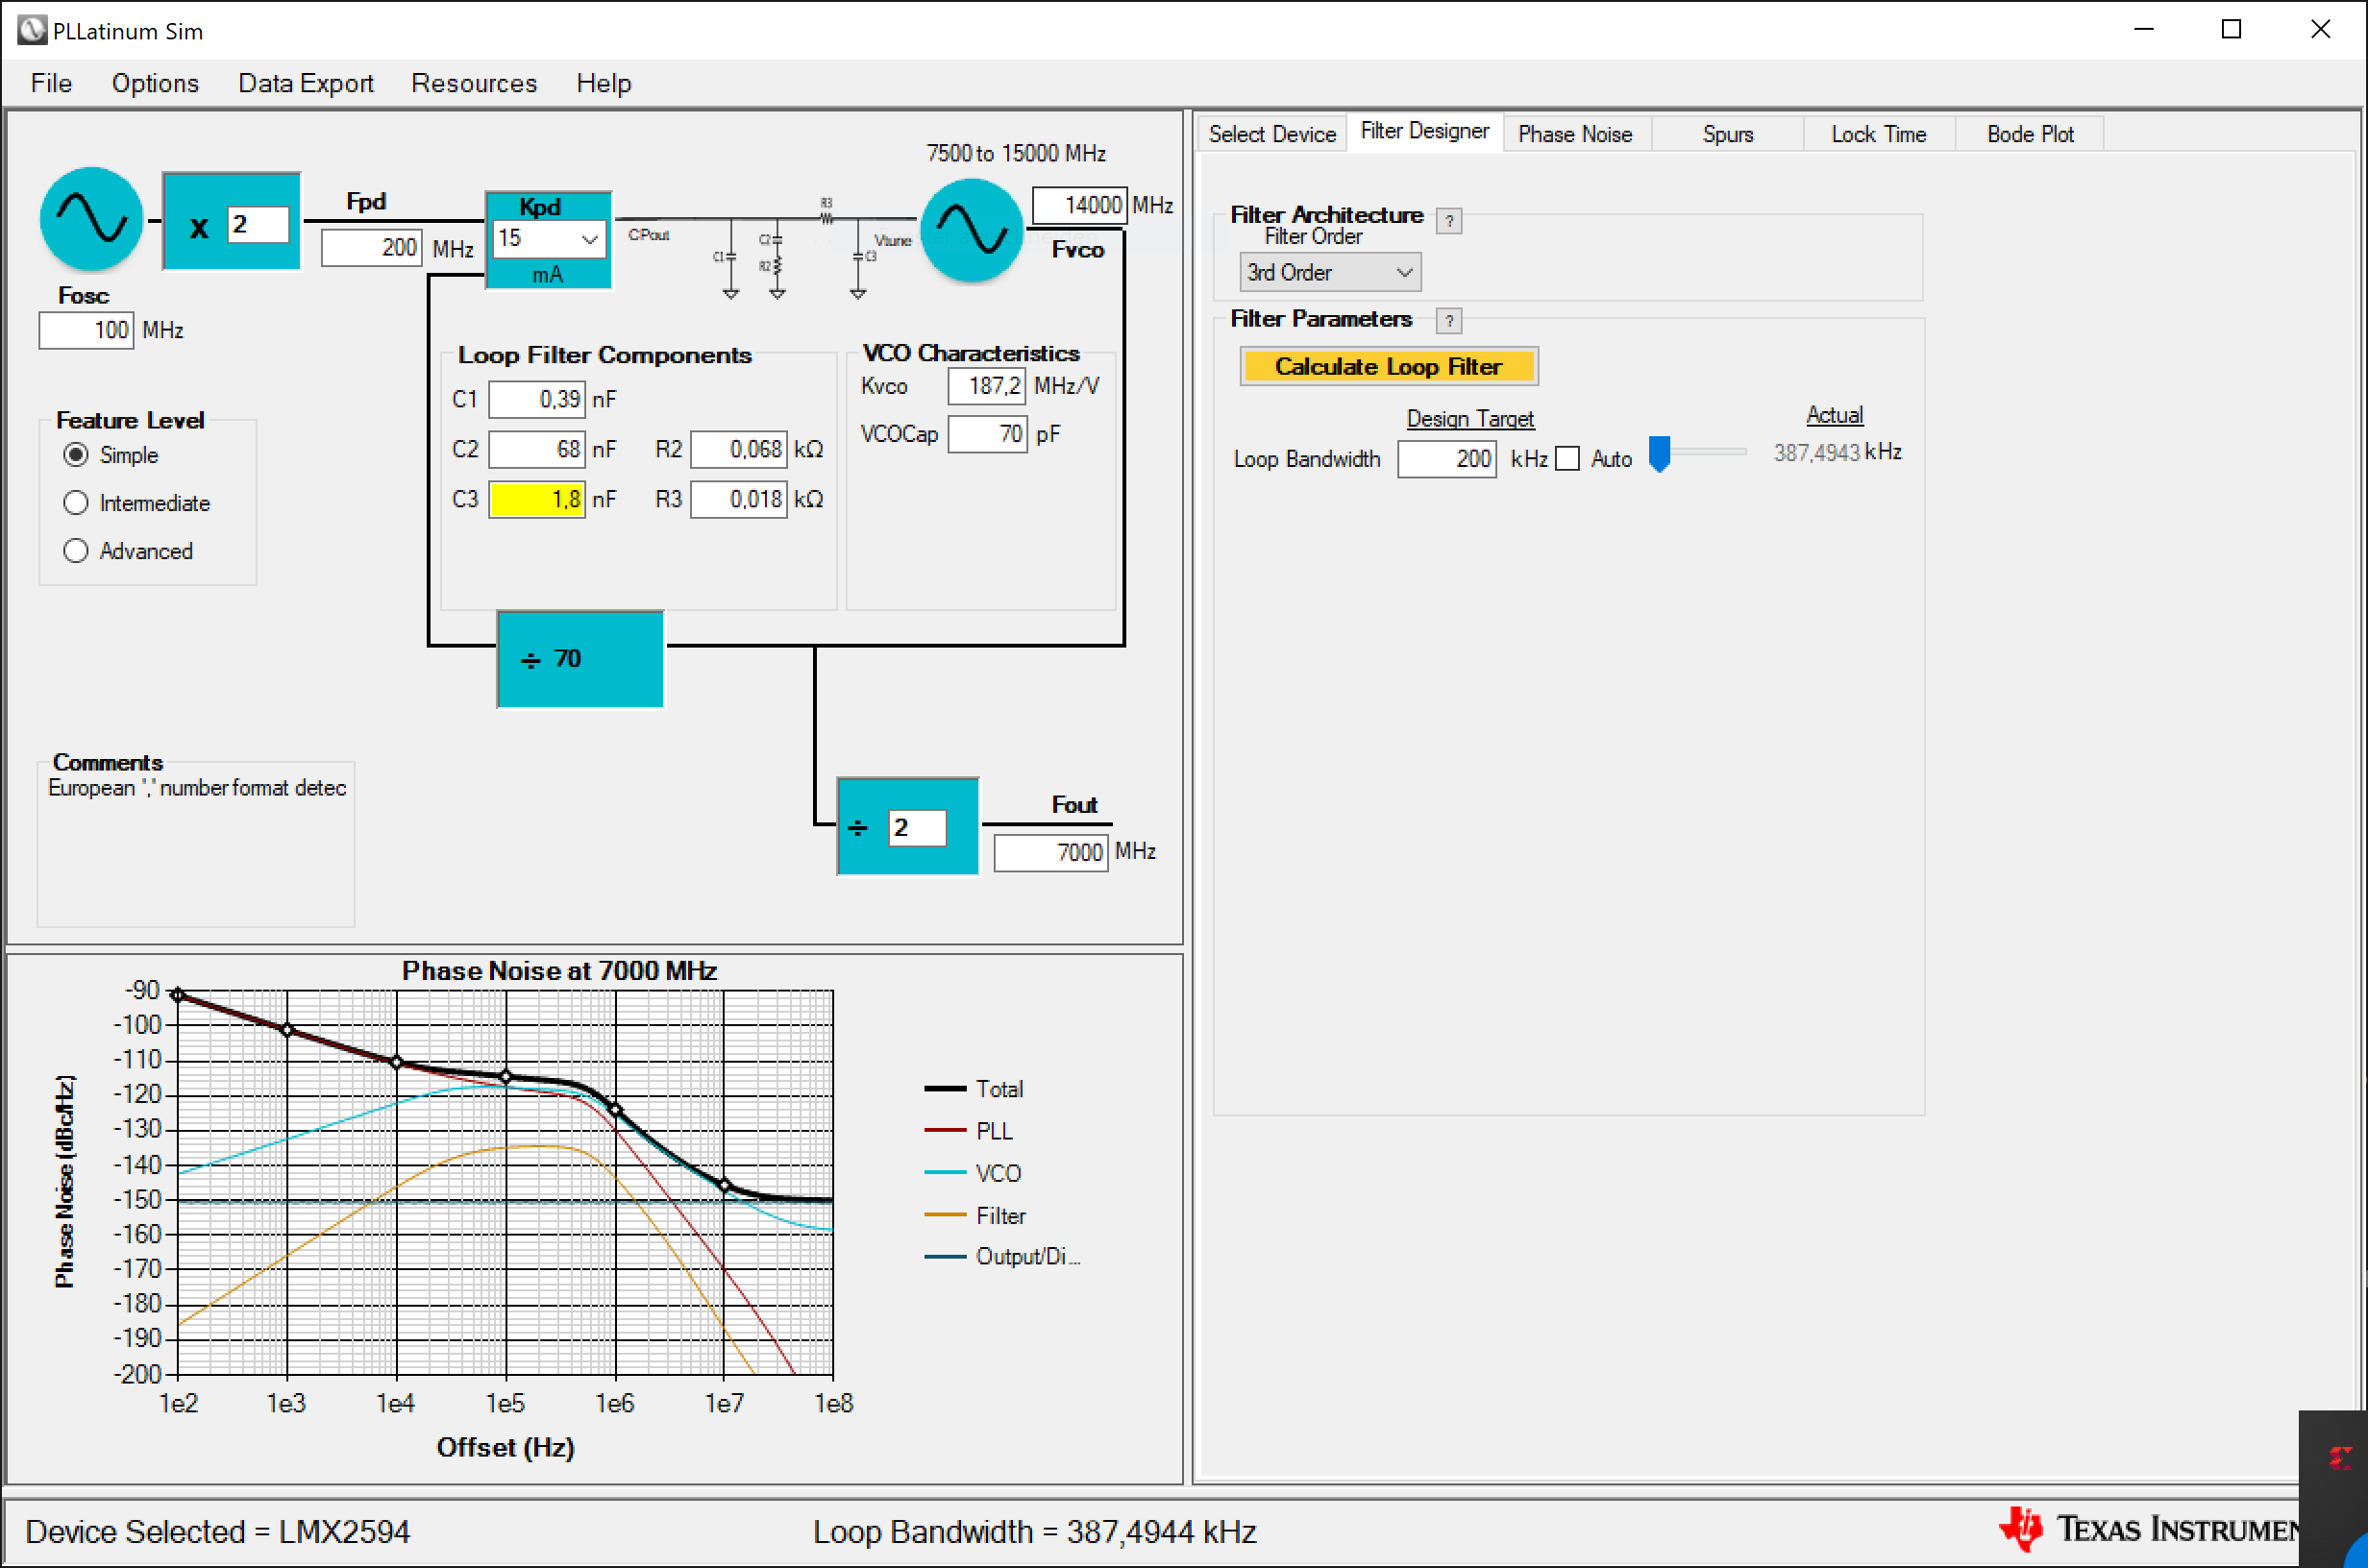
\includegraphics[height = 0.3\textwidth, width = 0.6\textwidth]{chap/03-work/img/pll.tikz}
	\caption{Schema with PLL. Red: only in "time-stretch-mode"}
	\label{fig:pll}
\end{figure}